\documentclass{article}
\pdfpagewidth=8.5in
\pdfpageheight=11in

\usepackage{WEDTreport}
% Use the postscript times font!
\usepackage{times}
\usepackage{soul}
\usepackage{url}
\usepackage{xcolor}
\usepackage{polski}
\usepackage[polish]{babel}
\usepackage[utf8]{inputenc}
\usepackage[T1]{fontenc}
\usepackage[utf8]{luainputenc}
\usepackage[hidelinks]{hyperref}
\usepackage[utf8]{inputenc}
\usepackage{caption}
\usepackage{indentfirst}
\usepackage{graphicx}
\usepackage{amsmath}
\usepackage{siunitx}
\usepackage{booktabs}
\usepackage{subfig}
\usepackage{pgf-pie}

\urlstyle{same}

\title{Wprowadzenie do eksploracji danych tekstowych w sieci WWW\\ Odpowiadanie na pytania}

\author{
Maria Konieczka, Alicja Poturała, Jakub Sikora
\affiliations
numery albumów: 283410, 283415, 283418 \\
\emails
maria.konieczka.stud@pw.edu.pl, alicja.poturala.stud@pw.edu.pl, jakub.sikora2.stud@pw.edu.pl
}

\newcommand{\todo}[1]{\textcolor{blue}{\textbf{TO DO:} #1}}
\newcommand{\opracowanyartykul}[1]{\textcolor{teal}{\textbf{Artykuł:} #1\\}}

\begin{document}
\maketitle

\section{Wprowadzenie}
\label{sec:wprowadzenie}
Lorem ipsum dolor sit amet, consectetur adipiscing elit. In ultricies justo id elementum rutrum. Donec et diam turpis. Suspendisse mollis id enim a ultricies. Sed eleifend neque eu gravida elementum. Sed faucibus fermentum faucibus. Cras vitae vehicula orci, vitae convallis ante. Phasellus at odio ultrices, interdum lacus non, dignissim augue.

Quisque et mi sit amet ligula volutpat molestie eu in est. Sed dictum non augue eu ornare. Morbi tristique arcu ex, non dapibus lacus sollicitudin suscipit. Donec ante justo, vulputate vel lectus sed, lacinia pharetra libero. Nulla elementum erat augue, id porta lacus sagittis nec. Sed ultricies augue neque, a scelerisque lectus dictum ac. Sed fermentum faucibus sem vitae pretium. Morbi lobortis tortor vitae enim elementum aliquam. Aliquam mollis lacus eget ipsum dignissim, eget cursus tortor dapibus. Donec feugiat nunc ac placerat rhoncus. Vestibulum at tempus purus. Cras et pharetra orci, quis tempus augue.

Quisque non tortor metus. Vestibulum sem dui, tempor eu placerat non, pharetra eget metus. Vestibulum venenatis, est in aliquet placerat, mi tellus fermentum magna, ut congue ligula lectus placerat elit. Nullam id sollicitudin nisi. Suspendisse sodales hendrerit arcu posuere semper. Sed vel tortor accumsan, ullamcorper tortor eget, tincidunt nisl. Suspendisse auctor odio orci, pellentesque varius lectus gravida non. Aliquam in urna sed dolor sollicitudin euismod congue vitae risus. Ut malesuada massa massa. Suspendisse mollis et libero non eleifend. Duis at lobortis ante.

\begin{figure}[h]
    \centering
    
\includegraphics[width=\columnwidth]{./figures/example.png}
    \caption{Morbi in erat tristique, ullamcorper felis eget, auctor risus}
    \label{fig:example-figure}
\end{figure}

Nulla ullamcorper nunc et dui sagittis lobortis. Aliquam erat volutpat. Proin congue purus at sapien aliquam, vel blandit enim fringilla. Curabitur facilisis turpis at ullamcorper vestibulum. Morbi in erat tristique, ullamcorper felis eget, auctor risus. Sed augue turpis, auctor cursus leo in, lacinia finibus enim. Sed ac tortor ac felis dignissim ullamcorper vel ut neque. Duis at arcu tortor. Nunc eu tincidunt lacus. Donec vitae nibh arcu. Phasellus gravida rhoncus diam viverra vulputate.

Aenean odio erat, rhoncus in pharetra sit amet, volutpat ac metus. Nam interdum quam nibh, vel semper lectus luctus sit amet. Vivamus eu dui dolor. Quisque euismod magna in dignissim faucibus. Curabitur vulputate ex id leo posuere, sed finibus quam ornare. Etiam eget imperdiet metus. Morbi odio est, iaculis pellentesque cursus et, interdum id erat. Aliquam ultricies metus risus, eu rutrum mauris fringilla sed. Duis malesuada nisi ex, molestie tristique metus tempor et. Curabitur vel est ac libero bibendum euismod. Maecenas vitae vulputate nisl, dignissim vehicula ipsum. Proin lobortis luctus augue, vel elementum erat sagittis varius. Mauris elementum, turpis vel fermentum vestibulum, ex turpis mattis eros, ut vehicula lorem nunc blandit enim. Suspendisse eget vestibulum mauris. Aenean fermentum tellus sit amet nulla pellentesque fringilla.

Curabitur ut mauris dignissim, fermentum lectus et, lacinia ligula. Cras at turpis nibh. Suspendisse interdum ipsum sed purus suscipit, ac auctor metus pretium. Vestibulum eu nisl ut magna pellentesque eleifend quis sed tellus. Nulla viverra magna non massa malesuada posuere. Cras sollicitudin fringilla lectus eget faucibus. Nam ac sapien consequat, consequat metus vel, feugiat ipsum. Interdum et malesuada fames ac ante ipsum primis in faucibus. Nulla ornare lectus augue, eget dictum nulla fringilla non. Aliquam at mauris eget sapien ornare aliquam~\cite{book-without-title}.

\section{Przegląd literatury}
\label{sec:przeglad}

Podczas przygotowań przeanalizowane zostało w sumie piętnaście publikacji naukowych dotyczących systemów odpowiadania na pytania. Naszym celem było stworzenie jak najszerszego opisu trudności towarzyszących tworzeniu systemów QA oraz znalezienie rozwiązań dla typowych problemów. Aby stworzyć przekrój problemu należało znaleźć zarówno pozycje opisujące zagadnienia związane z systemami odpowiadającymi na pytania ogólnw, jak i na pytania z ograniczonych dziedziń. Jako że postanowiliśmy zmierzyć się ze stworzeniem systemu odpowiadającemu na pytania w języku polskim, konieczne było także znalezienie literatury opisującej specyfikę tych systemów.

\subsection{Systemy odpowiadające na pytania ogólne}\label{subsec:lit:op}

\opracowanyartykul{The structure and performance of Open-Domain QA System~\cite{moldovan-etal-2000-structure}}
W artykule \cite{moldovan-etal-2000-structure} przedstawiona została budowa i opisane najważniejsze aspekty systemu QA o nazwie LASSO. Składa się on z trzech etapów: przetwarzania pytania, indeksowania ustępów i przetwarzania odpowiedzi. 

Pierwszy etap ma za zadanie określić typ pytania, spodziewany typ odpowiedzi, określić tzw. answer focus oraz zbudować zapytanie na podstawie pytania. W kolejnym etapie, za pomocą stworzonego zapytania,  należy odnaleźć paragrafy zawierające odpowiedź na zadane pytanie. W ostatnim etapie należy wyodrębnić odpowiedź na pytanie w wybranym paragrafie.

Ważnym aspektem pierwszego etapu jest stworzenie zapytania do wyszukiwarki. W opisywanym systemie do tego celu można zastosować 8 heurystyk. Do zapytania dodają wyrazy z pytania, które spełniają następujące wymagania: słowa tworzące cytaty (oprócz stop-słów), nazwy własne, wyrazy tworzące grupę nominalną, wszystkie rzeczowniki i ich określenia przymiotnikowe, wszystkie czasowniki, wyraz stanowiący centrum pytania (tzw. question focus). Do stworzenia początkowego zapytania wykorzystywane są tylko początkowe warunki. Jeżeli wyszukiwarka zwróci zbyt małą lub dużą liczbę paragrafów, wykorzystuje się pozostałe heurystyki, aby dodać więcej słów do zapytania lub usuwa wyrazy z zapytania. 

Do wyszukania stosuje się silnik, bazujący na logice boolowskiej.  Powstał on na bazie silnika Zprise IR, który porównuje paragrafy bazując na podobieństwie kosinusowym. Po odnalezieniu fragmentów z potencjalnymi odpowiedziami, są one oceniane i sortowane ze względu na: taką samą sekwencję słów we fragmencie i zapytaniu, największej odległości pomiędzy słowami kluczowymi w paragrafie i liczby brakujących słów kluczy w paragrafie. 

Ostatni etap przetwarza znalezione fragmenty w celu stworzenia odpowiedzi na zapytanie. Do tego celu wykorzystywany jest zmodyfikowany Brill tagger. Parser umożliwia wyodrębnienie z paragrafów fragmentów będących potencjalnymi odpowiedziami na pytanie. Fragmenty te, tworzące okna odpowiedzi, są następnie oceniane pod względem:  odległości potencjalnej odpowiedzi od pozostałych słów kluczy w oknie, pasujących słów kluczy w oknie, liczby słów kluczy będących w tym samym zdaniu co kandydat na odpowiedź, liczby słów kluczy będących w tym samym poddrzewie wyprowadzenia co potencjalna odpowiedź, i najlepszy z~nich stanowi odpowiedź na pytanie\cite{moldovan-etal-2000-structure}.

\opracowanyartykul{Answerbus question answering system~\cite{zheng2002answerbus}}
AnswerBus~\cite{zheng2002answerbus} jest systemem odpowiadającym na pytania ogólne, bazującym na wyszkuiwaniu informacji, opartym o~analizę zdań. System przyjmuje pytania w~sześciu językach (angielskim, niemieckim, francuskim, hiszpańskim, włoskim i~portugalskim) oraz odpowiada po angielsku. Odpowiedzi wyszukiwane są w~ internecie, posiłkując się pięcioma różnymi wyszukiwarkami m.in. Google czy AltaVista.

Przedstawione rozwiązanie składa się z~kilku komponentów, przetwarzających liniowo otrzymane pytanie. W pierwszej kolejności pytanie trafia do modułu rozpoznającego język. Jeżeli pytanie jest sformułowane w języku angielskim to trafia ono bez modyfikacji dalej, pytania sformułowane w pozostanych językach są tłumaczone za pomocą internetowego translatora. Kolejnym krokiem jest analiza pytania w~celu wydobycia typu pytania. Znaleziony rodzaj pytania determinuje, które wyszukiwarki zostaną wykorzystane w kolejnym etapie. System selekcjonuje trzy z~pięciu rozważanych wyszukiwarek. Wybrane rozwiązania są następnie odpytywane o~specjalnie przygotowane zapytanie, a~następnie z~otrzymanych dokumentów tekstowych wybierane są zdania, potencjalnie zawierające odpowiedź na pytanie. Ostatnim krokiem jest ocena wybranych zdań i~zwrócenie najlepszych wyników użytkownikowi~\cite{zheng2002answerbus}.  

System AnswerBus, podobnie jak większość tego rodzaju rozwiązań, określa typ postawionego pytania. Oprócz oczywistych typów, na przykład pytaniu \emph{Jak daleko} przypodządkowany jest rodzaj \emph{odległość}, system stara się ocenić dodatkowe parametry między innymi oczekiwany rząd wielkości (w~odpowiedzi na przykładowe pytanie oczekujemy odległości w~kilometrach a~nie w~centymetrach). Stwierdzenie typu pytania, pozwala na dokładniejszy dobór wyszukiwarki, od bardzo ogólnej jak Google do specjalistycznych jak Yahoo News~\cite{zheng2002answerbus}.

Analiza odpowiedzi sprowadza się do oceny otrzymanego zdania na podstawie treści pytania. Oczekiwana odpowiedź powinna zawierać jak najwięcej wyrazów z~zapytania. Nie powinna jednak uwzględniać słów nie niosących informacji takich jak przyimkni, zaimki, spójniki czy okoliczniki. Do oceny odpowiedzi stosuje wzór~\ref{eqn:ocena-answerbus},gdzie $q$ to liczba pasujących słów pytania a~$Q$ to liczba wszystkich wyrazów w~odpowiedzi~\cite{zheng2002answerbus}.

\begin{equation}
\label{eqn:ocena-answerbus}
q \geq  \sqrt{Q - 1}  + 1
\end{equation}

Oprócz zliczania słów, system wykrywa powiązania pomiędzy rzeczownikami a~zaimkami i~w~momencie wykrycia zaimka dokonywane jest zastąpienie zamika odpowiadającym mu rzeczownikiem. Na ocenę wpływają również obecność synonimów słów kluczowych oraz pozycja wyniku w~wyszukiwarce~\cite{zheng2002answerbus}.

\opracowanyartykul{An analysis of the askmr question-answering system~\cite{brill2002analysis}}\label{askmr}
System AskMSR~\cite{brill2002analysis} jest systemem zajmującym się odpowiadaniem na pytania ogólne. W~tym celu przeszukuje on sieć WWW, wykorzystując różne internetowe wyszukiwarki. Celem autorów, było stworzenie systemu odpowiadającego na pytania, bez przeprowadzania zaawansowanej analizy lingwistycznej zarówno pytania,jak i~potenjalnych odpowiedzi. Głównym założeniem był fakt olbrzymiej redundancji odpowiedzi w~sieci WWW.

Zasadniczo, system składa się z~czterech modułów. Pierwszy z~nich na podstawie pytania buduje zapytania do wyszukiwarki internetowej. Każde z~zapytań, zawiera pewną część oryginalnego pytania. Im więcej wyrazów oryginalnego zapytania znajduje się w~przygotowanym zapytaniu, tym z~większą wagą będą brane pod uwagę otrzymane na nie odpowiedzi. Skonstruowane zapytania są wysyłane do wyszukiwarki internetowej. Dalsze moduły przetważają jedynie krótkie fragmenty dokumentów, tzw. \emph{snippety} oraz przesyłane są linki~\cite{brill2002analysis}.

Drugim komponent systemu AskMSR zajmuje się wyszukiwaniem \emph{n-gramów} w~zwróconych odpowiedziach. W~tekstach wyszukiwane są tylko unigramy, bigramy oraz trigramy. Każdy z~\emph{n-gramów} jest oceniany na podstawie wcześniejszej oceny zapytania. Do oceny wliczana jest również liczba unikalnych odpowiedzi zwróconych przez system zawierający dany \emph{n-gram}~\cite{brill2002analysis}.

Przygotowane \emph{n-gramy} są przekazywane do trzeciego modułu - filtrowania. Moduł filtrowania, na podstawie ręcznie przygotowanych filtrów opartych na~wyrażeniach regularnych, określa jeden z~siedmiu typów pytania, a~następnie filtruje \emph{n-gramy}, zawężając potencjalny zestaw odpowiedzi. Ostatnim elementem systemu jest moduł łączenia, który wiąże ze sobą nakładające się \emph{n-gramy}, sukcesywnie budując coraz większe zdania, których konstrukcja nie byłaby możlwia wyłącznie poprzez tworzenie \emph{n-gramów}. Ocena połączonych \emph{n-gramów} jest określana na podstawie wyżej ocenianego składnika. Łączenie odbywa się do momentu aż system nie będzie mógł połączyć żadynch odpowiedzi~\cite{brill2002analysis}.

Autorzy systemu zwracają uwagę, że najwiekszy wpływ na jakość zwracanych odpowiedzi mają wpływ moduły filtrowania oraz łączenia \emph{n-gramów}. System został przetestowany przy pomocy pytań TREC-9~\cite{voorhees2001trec}. Najbardziej problematyczne okazały się pytania rozpoczynające się od \emph{jak?}, natomiast najlepiej radził sobie z~pytaniami rozpoczynającymi się od \emph{kto?}, z~dużą liczbą typowych dla języka słów~\cite{brill2002analysis}.

\opracowanyartykul{Data-Intensive Question Answering~\cite{brill2001data}}
Pozycja \cite{brill2001data} opisuje wykorzystanie systemu AskMSR oraz AskMSR2 na konferencji TREC-9 w 2001 roku. Jako że analiza systemów została przedstawiona powyżej (pozycja \cite{brill2002analysis}), w opisie artykułu pominięte zostaną kwestie poruszone powyżej.

Główną modyfikacją systemów AskMSR oraz AskMSR na potrzeby konferencji TREC było dodanie fazy sprawdzającej wystąpnie potencjalnej odpowiedzi w zbiorze dokumentów TREC. System po znalezieniu n najlepszych odpowierdzi z zasobów internetowych, wyszukiwał ich w bazie danych TREC-9. W tym celu wykorzystany został system Okapi IR. Zapytanie polegało na stworzeniu query skłądającego się ze słów użytych w potencjalnej odpowiedzi. Znalezione dokumenty były następnie poddawane ocenie.

Autorzy \cite{brill2001data} na tym etapie generacji odpowiedzi nie wykorzystywali specjalnych zabiegów lingwistycznych w celu zwiększenia precyzji ani pokrycia. Do dalszego przetwarzania wybierane były najwyżej ocenione dokumenty dla każdej z potencjalnej odpowiedzi.

Ostateczne odpowiedzi systemu były w większości przypadków generowane na podstawie najwyżej ocenianych dokumentów wspierających potencjalne odpowiedzi. Wyjątkiem od reguły była sytuacji, gdzie jeden dokuemnt powtarzał się w kilku potencjalnych odpowiedziach.

Autorzy \cite{brill2001data} zwracają uwagę, że mechanizm ten może być wykorzystywany także w innych zastosowaniach. Wskazują, że można go wykorzystać do weryfikacji potencjalnej odpowiedzi znalezionej w internecie w niewielkich, ale wiarygodnych zbiorach takich jak słowniki lub bazy arykułów \cite{brill2001data}.

\opracowanyartykul{IBM's Statistical Question Answer System~\cite{Ittycheriah00ibm'sstatistical}}
W artykule \cite{Ittycheriah00ibm'sstatistical} zaprezentowana została ogólna budowa systemu IBM, który wykorzystuje klasyfikator maksymalnej entropii do określania rodzaju pytania oraz typu spodziewanej odpowiedzi, a także do oznaczania klasy bytów występujących w tekście. 

System składa się z czterech głównych modułów: klasyfikacji rodzaju pytania i odpowiedzi, rozszerzenia zapytania/wyszukiwania informacji, oznaczania klasy bytów występujących w wyszukanym tekście (named entity marking), wyboru odpowiedzi. 

W systemie, określenie typu odpowiedzi polega na przyporządkowaniu do pytania etykiety określającej szukany byt. Do określenia typu bytu, autorzy korzystają z kategorii MUC, opisanej w artykule \cite{chinchor-robinson-1998-appendix}, lub przyporządkują typ PHRASE, gdy typu nie da się określić. Za przyporządkowanie tych etykiet odpowiada model maksymalnej entropii. 

Drugim opisanym aspektem systemu był moduł wyszukiwania informacji. Autorzy proponują podejście dwuetapowe. Pierwszy etap polega na przeszukaniu bazy danych encyklopedii. Wyszukane fragmenty są oceniane za pomocą schematu Okapi opisanej w artykule \cite{RobertsonOkapi}. Ustępy o najwyższym wyniku są następnie użyte do rozszerzenia zapytania za pomocą techniki LCA. Drugi etap polega na wyszukaniu w korpusie TREC-9 rozszerzonego zapytania.

Przedostatnim modułem jest oznaczenie klasy bytów występujących w wybranych ustępach. Klasyfikator maksymalnej entropii przyporządkuje każdemu słowu kategorię MUC \cite{chinchor-robinson-1998-appendix}. Tak zmodyfikowany ustęp wraz z spodziewanym typem odpowiedzi stanowi wejście do ostatniego modułu.

Każdy ustęp przekazany do ostatniego modułu dzielony jest na zdania. Wokół każdego zdania formowane jest okno. Każde okno jest oceniane na podstawie pięciu parametrów. Dodatkowo brana pod uwagę jest obecność lub brak spodziewanego typu odpowiedzi. Na koniec wybieranych jest 50 lub 250 bajtów najbardziej dopasowanych okien\cite{Ittycheriah00ibm'sstatistical}. 

\opracowanyartykul{Question-answering systems: Developement and prospects~\cite{lapshin2012question}}
W pracy~\cite{lapshin2012question} przedstawiona została ogólna struktura systemu do odpowiadania na pytania ogólne. Autor podzielił proces odpowiadania na kilka odrębnych faz:
\begin{itemize}
	\item określanie typu pytania,
	\item przetwarzanie pytania,
	\item określenie kontekstu,
	\item przeszukiwanie bazy wiedzy,
	\item konstruowanie odpowiedzi.
\end{itemize}

Oprócz tego, w~pracy zostały określone obostrzenia, które powinien spełniać system:
\begin{itemize}
	\item interaktywność,
	\item odpowiadanie w~czasie rzeczywistym,
	\item logiczne wnioskowanie,
	\item profilowanie użytkownika,
	\item odpowiadanie w~różnych językach.
\end{itemize}

Przykładowym systemem, spełniającym przedstawione wymagania, jest \emph{DeepQA}, znany obecnie pod nazwą \emph{IBM Watson}. W~pierwszym etapie przetwarzania, system analizuje pytania, określając jego klasę, typ oczekiwanej odpowiedzi oraz buduje związki logiczne pomiędzy wyrazami w~pytaniu. Dzięki temu, jest on w~stanie zbudować odpowiednie zapytanie do bazy wiedzy, którą w~tym przypadku jest sieć WWW. W~kolejnym kroku, \emph{Watson} tworzy hipotezy odpowiedzi, które następnie sprawdza, poszukując dowodów oraz dokonując analizy krytycznej źródeł. Ostatecznie, ze zbioru odpowiedzi wybierana jest ta najbardziej prawdopodobna i~to ona zostaje zwrócona użytkownikowi~\cite{lapshin2012question}.

Najważniejszym elementem całego systemu jest moduł klasyfikacji odpowiedzi. Poprawna klasyfikacja jest odpowiedzialna za największy przyrost poprawnych odpowiedzi. System korzysta ze zbioru kategorii pytań, nazywany ontologią. Pierwsze zbiory określały od 13 do 18 kategorii pytań, natomiast w~późniejszych pracach, zaczęto dzielić kategorię na kategorię główne i~szczegółowe, przykładowo w~\cite{li2002learning} określono sześć typów głównych i prawie pięćdziesiąt typów szczegółowych. Do określania typu pytania najczęściej wykorzystywane są klasyfikatory regułowe oraz statystyczne. Tego typu naiwne podejście jest bardzo proste i~daje dobre rezultaty~\cite{lapshin2012question}.

To co pozwala dobrze oceniać system \emph{IBM Watson} to nie tylko dobre wyniki w~testach na pytaniach z~konferencji TREC, ale również potężny sukces biznesowy, który firma IBM osiągnęła sprzedając swoje rozwiązanie\footnote{https://www.ibm.com/watson}. W~połączeniu z~otwartą chmurą, nowoczesne przedsiębiorstwa mogą wykorzystać Watsona do tworzenia inteligentnych systemów zarządzania oraz wspierania ludzi w~przemyśle, medycynie i~logistyce. Najbardziej znanym przykładem użycia systemu \emph{IBM Watson} jest jego udział w~programie \emph{Jeopardy!}, w~którym to uczestnicy odpowiadają na zróżnicowane i~skomplikowane pytania~\cite{lapshin2012question}. 

\opracowanyartykul{Learning Surface Text Patterns for a Question Answering System~\cite{ravichandran-hovy-2002-learning}}
Artykuł \cite{ravichandran-hovy-2002-learning} poświęcony jest tematyce wykorzystania wzorców tekstowych w systemach QA. Autorzy zauważają, że odpowiedzi na większość pytań można zlokalizować w tekście poprzez znalezienie charakterystycznych wzorców. Przykładowo, aby odszukać rok urodzenia danej osoby, należy odnaleźć tekst pasujący do wzorca: “<NAME> was born in <BIRTHDATE>”.

Artykuł skupia się na temacie automatycznej generacji wzorców oraz ocenie ich precyzji. Autorzy prezentują algorytm, który samodzielnie tworzy wzorce na podstawie pary: wyraz-pytanie (question term)i wyraz-odpowiedź (answer term). 

Aby stworzyć wzorzec należy dla danego typu pytania (np. BIRTHYEAR), wyszukać w zbiorze tekstów zdania zawierające wyraz-pytanie i wyraz-odpowiedź  – przykładowo „Mozart 1756”. Ze znalezionych zdań buduje się drzewa sufiksowe, aby znaleźć wszystkie podciągi zdania o różnych długościach. Te podciągi, które zawierają zarówno wyraz-pytanie i wyraz-odpowiedź, tworzą wzorzec (<NAME> was born on <ANSWER>). Algorytm można usprawnić wprowadzając rozszerzenie, które pozwala na określenie spodziewanej długości odpowiedzi dla niektórych typów pytań. 

Autorzy przetestowali tworzenie wzorców przy wykorzystaniu korpusu TREC oraz wyszukiwarki internetowej. Z~uwagi na redundancję danych, większą precyzję osiągnęły wzorce stworzone na podstawie tekstów z internetu. 

Wśród wad wykorzystania wzorców tekstowych, autorzy wymieniają ignorowanie informacji na temat typu spodziewanej odpowiedzi. Do wzorca może zostać dopasowany każdy pasujący zwrot bez względu na typ części mowy. Kolejną wadą jest zagrożenie powstania zbyt ogólnikowych wzorców w przypadku niektórych pytań. Problem ten występuje między innymi w przypadku pytań o definicję. Autorzy podkreślają także istotną wagę odpowiedniego doboru przykładów (wyraz-pytanie i wyraz-odpowiedź), na podstawie których tworzone są wzorce oraz potrzebę korzystania z dużej bazy tekstów. Podejście z dopasowywaniem wzorców, nie sprawdza się najlepiej przy tekstach, w których pytanie i odpowiedź znajdują się w dalekiej odległości od siebie (“<QUESTION>, (<dużo wyrazów>)*, lies on <ANSWER>”). Poważnym ograniczeniem metody jest także to, że może być stosowana tylko do pytań o jednym wyrazie-pytania. Przykładowo w pytaniu “Which county does the city of Long Beach lie?” są dwa wyrazy-pytania: „county” i „Long Beach”, dlatego algorytm zaproponowany przez autorów nie sprawdzi się. Problemem jest także występowanie różnych form danego zwrotu (Gandhi może zostać zapisany także jako “Mahatma Gandhi”, “Mohandas Karamchand Gandhi) czy różnych form zapisu. 

Zaletą tej metody jest natomiast to, że można ją wykorzystywać dla wielu języków, ponieważ nie bierze pod uwagę cech specyficznych dla danego języka\cite{ravichandran-hovy-2002-learning}.

\opracowanyartykul{High Performance Question/Answering~\cite{hpqa}}
W artykule \cite{hpqa} opisano charakterystyczne aspekty systemu Question/Answer, dzięki którym system cechuje się wysoką dokładnością przy odpowiadaniu na pytania. Autorzy przekonują, że na skuteczność systemu QA wpływa nie tylko rozpoznawanie typu spodziewanej odpowiedzi, ale także zmiany leksykalne, morfologiczne i semantyczne przeprowadzone na słowach kluczowych.

Pierwszym ważnym aspektem systemu Question/Answer jest stworzona przez autorów taksonomia odpowiedzi (ANSWER TYP TAXONOMY), która umożliwiła znaleźć spodziewany typ odpowiedzi dla większości zapytań. Każdy węzeł w stworzonej taksonomii połączony jest z jedną lub więcej pod-hierarchii bazy WordNet. 

Aby znaleźć odpowiednią kategorię za pomocą tej taksonomii, należy przeprowadzić operację na zapytaniu, aby określić który wyraz determinuje typ spodziewanej odpowiedzi. W tym celu autorzy zaimplementowali własną wersję parsera Collinsa, która z zapytania tworzy drzewo wyprowadzenia (ang. parse tree). Znaleziony korzeń drzewa zmapowany na odpowiednie pojęcie w stworzonej taksonomii odpowiedzi stanowi spodziewany typ odpowiedzi. 

Otrzymane drzewo służy także autorom do skonstruowania zapytania do wyszukiwarki, ponieważ można z niego odczytać zależności pomiędzy słowami w pytaniu i stworzyć listę uporządkowaną. Uporządkowane w kolejności słowa z listy tworzą zapytanie. 

Kolejną cechą charakterystyczną dla systemu Q/A jest występowanie pętli przy wyszukiwaniu fragmentów z potencjalnymi odpowiedziami. Jeżeli w odpowiedzi na dane zapytanie znaleziono zbyt małą lub zbyt dużą liczbę paragrafów, pętla pozwala na powrót do tworzenia zapytania, w celu zwiększenia lub zmniejszenia liczby słów w zapytaniu. Następnie sprawdzane jest podobieństwo w zależnościach pomiędzy pytaniem a potencjalną odpowiedzią. Jeżeli podobieństwo jest niewystarczające, druga pętla pozwala na zmiany leksykalne, morfologiczne lub znaczeniowe w zapytaniu. 

Innym podejściem do odnalezienia paragrafów z potencjalnymi odpowiedziami opisanym w artykule było wykorzystanie modelu perceptronu. Do jego nauki posłużyły pary ustępów: pierwszy zawierający prawidłową odpowiedź, drugi będący paragrafem otrzymanym przy wykorzystaniu pętli.

Ostatnią opisaną właściwością systemu było szukanie podobieństwa pomiędzy zadanym pytaniem, a pytaniami zadanymi w przeszłości. Jeżeli podobne pytanie występowało w~przeszłości, tworzy się grupę zawierającą oba pytania\cite{hpqa}.

\opracowanyartykul{A survey of Text Question Answering Techniques~\cite{gupta2012survey}}
Według~\cite{gupta2012survey}, proces automatycznego odpowiadania na pytania można podzielić na trzy oddzielne fazy: klasyfikację pytania, wydobycie informacji z~bazy wiedzy oraz wydobycie/generację odpowiedzi. Te trzy fazy są wyróżnialne w~każdym systemie do odpowiadania na pytania, niezależnie od wykorzystanego mechanizmu. Autorzy wyodrębnili cztery różne podejścia do rozwiązania postawionego problemu, wyróżniając systemy oparte~o:
\begin{itemize}
	\item przeszukiwanie sieci WWW,
	\item wyszukiwanie w~bazie dokumentów tekstowych,
	\item wyszukiwanie w~zamkniętej bazie danych,
	\item reguły i~dopasowywanie do wzorca.
\end{itemize}

Autorzy podkreślają jak ważne jest automatyczne wydobycie informacji z~przygotowanego dokumentu. W~celu poprawnego wydobycia poszukiwanych informacji z~dokumentu należy w~pierwszej kolejności dokonać filtrowania akapitów. Zazwyczaj dokonuje się tego wykorzystując dopasowywanie do słów kluczowych zapytania. Im więcej razy w~tekście wystąpi słowo kluczowe, tym większa szansa na to że nie zostanie ono odfiltrowane. Następnie, każdemu pozostałemu akapitowi należy przyporządkować liczbę określającą jakość tekstu.
Dobór funkcji oceniającej jest zależny od typu przetwarzanych dokumentów oraz rodzaju pytania. Ocenione akapity należy posortować a~następnie, rozpoczynając od pierwszego, przeprowadzić proces leksykalnego i~syntaktycznego wydobycia wiedzy z~tekstu~\cite{gupta2012survey}.

Aby odpowiednio ocenić akapity, należy przed przetwarzaniem dokumentów dokonać klasyfikacji pytania. Autorzy~\cite{gupta2012survey} wyodrębnili osiem klas głównych pytań odpowiadających na pytania:
\begin{itemize}
	\item co?,
	\item jak?,
	\item dlaczego?,
	\item który/która/które/którzy?,
	\item gdzie?,
	\item czyji/kogo?
	\item kiedy?,
	\item pytania funkcjonalne.
\end{itemize}

Wykorzystanie reguł logicznych oraz wyrażeń regularnych w prosty sposób umożliwia rozróżnienie piereszych siedmiu klas. Największą trudność sprawiają pytania funkcjonalne typu \emph{Nazwij piłkarza który strzelił jedyną bramkę w~finale Euro 2016}. Pytania tego typu wymagają szczególnego traktowania i~najczęściej wymagają maszynowego rozumienia tekstu\cite{gupta2012survey}.

\subsection{Systemy odpowiadające na pytania dziedzinowe}\label{subsec:lit:res}

\opracowanyartykul{A Practical QA System in Restricted Domains~\cite{restrictedWeather}}
Artykuł ~\cite{restrictedWeather} przedstawia opis systemu odpowiadającego na pytania, który został stworzony dla robota pracującego w~warunkach domowych. Autorzy zauważyli, że systemy tego typu znajdują swoje zastosowanie w~ograniczonych dziedzinach takich jak pogoda czy program stacji telewizyjnych oraz, że dla użytkowników takich systemów znacznie ważniejsza jest precyzja uzyskanych odpowiedzni. Artykuł skupił swoją uwagę na opisie systemu umożliwiającemu znalezienie odpowowiedzi na pytania związane z pogodą. 

Proces odpowiadania na pytania jest trójfazowy. Składa się on z: 
\begin{itemize}
	\item przetworzenia zapytania w języku naturalnym na zapytanie SQL,
	\item realizacji zapytania,
	\item konwersji otrzymanego rezultatu na język naturalny.
\end{itemize}
Stworzony system zbudowany jest z trzech modułów: 
\begin{itemize}
	\item silnika IE, 
	\item DBMS, 
	\item silnika QA.
\end{itemize}

Dane wykorzystywane do znalezienia odpowiedzi na pytania pochodzą z~wybranych przez autorów, połowicznie ustrukuryzowanych stron internetowych narodowego instytutu meteorologicznego Korei Południowej. Silnik IE co godzinę pobiera z~odpowiedniej strony internetowej najnowsze dokumenty, parsuje je i wydobywa zdyskretyzowane informacje o aktualnych warunkach meteorologicznych, które to następnie są zapisywane w bazie danych. 

Silnik QA służy do analizowania zapytań oraz konwertowania uzyskanych odpowiedzi na język naturalny. Autorzy \cite{restrictedWeather} wydzielili skończoną liczbę tematów (związanych z pogodą) o~jakie może zapytać użytkownik. Są to między innymi: temperatura powietrza, prędkość wiatru, opady. Analiza pytania polega na ekstrakcji słów kluczowych dotyczących m.in.: tematu pytania, miejsca, czasu. Aby móc zidentyfikować dokładnie intencje człowieka, przy użyciu specjalnego modułu, wyszczególnione z~zapytania słowa kluczowe są konwertowane na konretne terminy stosowane w systemie. Dzięki temu pytanie o konieczność wzięcia parasola jest traktowane tak samo jak pytanie czy pada aktualnie deszcz. W~kolejnym etapie przetwarzania pytania system zamienia wyrażenia czasowe takie jak \textit{dzisiaj} i~\textit{jutro} na wartości bezwzględne.

Autorzy \cite{restrictedWeather} zwrócili uwagę na fakt, że użytkownicy robotów domowych przy zadawaniu pytań często pomijają niektóre informacje związne~z lokalizacją i~czasem. Z~tego powodu system wykorzystuje stworzony profil użytkownika by uzupełnić brakujące informacje.

Tak przetworzone dane są wejściem dla klasyfikatora drzewiastego, którego zadaniem jest przyporządkowanie pytania do konkretnego, zdefioniowanego przez autorów query. Każdemu liściowi drzewa decyzyjnego przypisany jest konkretny schemat zapytania SQL oraz konkretny schemat odpowiedzi. System odrzuci pytanie, jeśli klasyfikator nie przyporządkuje pytaniu żadnego query.

Przedstawiony przez autorów \cite{restrictedWeather} system został przetestowany przez 10 osób i~ zostało zadane łacznie 50 pytań. Uzyskano $\num{90.9}$\% poprawnych odpowiedzi, podczas gdy pokrycie wyniosło $\num{75}$\%. Należy jednak zwrócić uwagę na ograniczenia i~sposób działania systemu. Pobiera on dane tylko ze zdefiniowanych przez autorów stron internetowych oraz generowane odpowiedzi są schematyczne~\cite{restrictedWeather}.

\opracowanyartykul{Aqualog: An ontology-portable question answering system for the semantic web~\cite{lopez2005aqualog}}
Artykuł \cite{lopez2005aqualog} opisuje ogólną architekturę oraz sposób działania systemu Aqualog. System ten umożliwia wyszukiwanie odpowiedzi na pytania w sieciach semantycznych. Stworzony został dla ontologii związanej z życiem akacemickim, ale autorzy podkreślają, że zaimplementowane metody w prosty sposób można przenieść do innych ontologii.

Proces przetwarzania zapytania przez system Aqualog można przedstawić za pomocą modelu waterfall. Zapytania użytkownika w kolejnych krokach przetwarzane są najpierw do trójek-query a następnie do trójek dostosowanych do ontologii. Na samym początku za pomocą ifrastruktury GATE system wykrywa części mowy poszczególnych słów użytych w zapytaniu. Znalezione adnotacje zawierają mniędzy innymi informacje o częściach zdaniach, tokenach, wykrytych rzeczownikach i~czasownikach. System został rozszerzony o~zbiór adnotacji dotyczących relacji, wzorów, typów pytań. Całość składowana jest za pomocą wykorzystania gramatyki JAPE a~wynikiem tego procesu są trójki-query.

Tak przetworzone dane stanowią wejście do serwisu podobieństw relacji (ang. Relation Similarity Service). Jest to serce systemu, które na podstawie znajomości struktury ontologii oraz dodatkowych infromacji stara się znaleźć odpowiednią trójkę dostosowaną do danej ontologii. Za pomocą RSS oraz serwisu podobieństwa klas (ang. Class Similarity Service) identyfikowane oraz mapowane są relacje i~nazwy w~ramach danej ontologii. Serwis wykorzystuje zarówno znajomość danej ontologii jak również mechanizm uczenia, aliasy zwrócone przez WordNet oraz korzysta z heurystyk.

CSS wykorzystywany jest do mapowania terminów lingwistycznych do klas. Używany jest w tym celu algorytm mierzący odległość pomiędzy napisami (ang. string distance metric). Dodatkowo serwis może wykorzystywać synonimy (znalezione za pomocą WordNet) lub mechanizmy uczenia się. 

Największymi trudnościami z jakimi powinien radzić sobie system są niejednoznaczoności. Autorzy założyli, że ta część systemu jest interaktywna, użytkownik proszony jest o doprecyzowanie znaczenia słów, których system nie potrafi jednoznacznie sklasyfikować. Dodatkowe, wprowdzone przez użytkownika, informacje są zapamiętywane zgodnie z kontekstem w jakim się pojawiły. Dzięki temu system ma zdolność uczenia się. Kontekst składa się między innymi z nazwy relacji, jej argumentów oraz informacji o użytkowniku. Jeśli w kolejnych zapytaniach serwis RSS nie znajdzie odpowiedniej trójki dostosowanej do ontologii, sprawdzane jest, czy w~bazie danych nie znajdują się zapamiętane wcześniej wyrażenie z takim samym kontekstem. Wykorzystywane są dwa podejścia: uczenie się oraz dopasowywanie.

Znalezione przez RSS trójki bezpośrednio wykorzysywane są do odnalezienia informacji w sieciach semantycznych. Autorzy wskazują na duże podobieństwa systemu Auqalog z systemami przetwarzającymi język naturalny na potrzeby analizy zapytań relacyjnych baz danych\cite{lopez2005aqualog}.

\opracowanyartykul{An English language question answering system for a large relational database~\cite{waltz1978english}}
Pozycja \cite{waltz1978english} opisuje sposób działania oraz budowę systemu odpowiadania na pytania PLANES. System ten został stworzony w celu zapewnienia wygodnego interfejsu do bazy danych związanej z samolotami dla amerykańskiego wojska w~drugiej połowie lat 70-tych ubiegłego wieku.

Artykuł \cite{waltz1978english} opisuje budowę całego systemu (wliczając w~to budowę stworzonej relacyjnej bazy danych), ale z perspektywy tworzenia nowego systemu QA istotne są tylko kwestie związane z konstrukcją parsera. Przetwarzanie zapytania składa się z czterech etapów: parsowania pytania, konstrukcji odpowiedniego query, dokonania jego oceny oraz wykonania zapytania i zwrócenia odpowiedzi. Założenia z jakich wyszli autorzy systemu to: wykorzystywanie specyficznego słownictwa przez użytkowników, a co za tym idzie brak dwuznaczności oraz fakt, że użytkownicy systemu nie tworzą długich zapytań.

System podzielił parsowanie pytania na kilka etapów. W~pierwszym dokonywana była poprawa literówek oraz konwersja słów do ich kanonicznych postaci. W drugim etapie wykorzystywane były podsieci ATN, których zadaniem było połączenie frazy ze zdefiniowanym w systemie znaczeniem. Dla każdego rodzaju obiektu (na przykład czas, rodzaj samolotów, rodzaj usterek) zaimplementowana została osobna podsieć rozpoznająca znaczenie słowa. 

Zaletą systemu było szybkie odrzucanie słów nie niosących żadnej informacji, które przez autorów \cite{waltz1978english} zostały nazwane szumami. Identyfikowane one były za pomocą osobnej podsieci. 

System, jeśli udało mu się znaleźć znaczenie jednego słowa używając danej podsieci, starał się wykorzystać ją ponownie w procesie identyfikacji następnego słowa.

Po przeanalizowaniu wszystkich słów oraz odrzuceniu szumów system aktualizował rejestr kontekstu, który został zaimplementowany w postaci stosu. W rejestrze tym znajdują się ostatie zapytania wraz z ostatnio wykrytymi frazami, ostatnio użytymi query oraz znalezionymi odpowiedziami. Do rejestru zostały wrzucane w tej fazie parsowania kanoniczne formy słów wraz z ich znaczeniem. Rejestr ten gra istotną rolę w procesie ustalania niesprecyzowanych zmiennych. Służy między innymi do znajdowania właściwych znaczeń zaimków.

Jeśli system nie jest w stanie jednoznaczie odtworzyć znaczenia danego słowa, to tworzone są struktury zwane ramkami pojęć (ang. concept case frames). Struktura składa się z~czasownika oraz części rzeczownikowych, do każdej przypisany jest wzór query. System testuje struktury oraz sprawdza, czy ich wykorzystanie może mieć sens. Jeśli wynik testowania jest pozytywny dla większej niż jednej struktury, użytkownik proszony jest o wybranie pożądanego znaczenia ze stworzonych przez system ramek.

Tak stworzone struktury przekzywane są następnie do modułu tworzącego zapytania. Proces tworzenia zapytania rozpoczyna się od próby identyfikacji tablic potrzebnych do znalezienia danych. Następnie moduł sprawdza jakiej odpowiedzi oczekuje użytkownik, czyli jakiej domeny powinien być zwrócony wynik. Jako że system był tworzony w latach 70-tych, dużym wyzwaniem było przetważanie złożonych zapytań.

Przed rozpoczęciem realizacji zapytania, PLANES przekazywał użytkownikowi stworzone query oraz umożliwił wprowadzanie korekt. Dane zwrócone z bazy danych były przekazywane do generatora odpowiedzi, który na podstawie rodzaju zwróconych danych oraz polecenia użytkownika konwertował je do postaci grafu lub tabeli\cite{waltz1978english}.

\subsection{Systemy odpowiadające na pytania w języku polskim}\label{subsec:lit:pl}


\opracowanyartykul{Issues of polish question answering~\cite{przybyla2012issues}}
W~pracy~\cite{przybyla2012issues}, autor opisuje budowę typowego systemu do odpowiadania na pytania otwarte, porównując które elementy takiego rozwiązania są zależne od języka. Oprócz tego, podkreślone zostały cechy języka polskiego, jako języka słowiańskiego, które utrudniają automatyczne przetwarzanie oraz generację tekstu.

Główną cechą czyniącą przetwarzanie tekstów w~języku polskim trudnym, jest mnogość form językowych. Fleksyjność języków słowiańskich pozwala na określanie roli wyrazu w~zdaniu na podstawie końcówki, a~nie jak w~języku angielskim na podstawie pozycji w~zdaniu. Przykładowo zdanie \emph{Jan zjadł rybę} oraz \emph{Rybę zjadł Jan}, znaczą to samo, mimo inaczej położonego akcentu, natomiast zdania \emph{John ate a~fish} i~\emph{A~fish ate John} znaczą zupełnie co innego. Co więcej, złożona odmiana rzeczowników sprawia że rozpoznawanie nazw własnych jest jeszcze trudniejsze~\cite{przybyla2012issues}.

Jako komponenty zależne od języka, autor wydzielił:
\begin{itemize}
	\item przetwarzanie bazy wiedzy,
	\item przetwarzanie pytania,
	\item generacja odpowiedzi,
	\item rozwijanie anafor.
\end{itemize}

W~przypadku przetwarzania bazy wiedzy, autor podkreśla że klasyczny \emph{stemming} nie zdaje egzaminu oraz że o~wiele lepsze wyniki uzyskuje się przy użyciu pełnych analizatorów morfologicznych, które przetwarzają tekst wolniej jednak gwarantują znalezienie każdej formy językowej dla przetwarzanego segmentu.

Mimo wielu różnic, autor podkreśla że kilka operacji, skutecznie używanych w~systemach do odpowiadania w~języku angielskim, może sprawdzić się w~systemach obsługujących język polski. Taką operacją jest między innymi indeksowanie bazy wiedzy, w~celu przyspieszenia wyszukiwania tekstu oraz wyszukiwanie relacji pomiędzy wyrazami, wykorzystując narzędzia typu \emph{WordNet}\cite{przybyla2012issues}.

\opracowanyartykul{Question Analysis for Polish Question Answering~\cite{przybyla-2013-question}}
Artykuł \cite{przybyla-2013-question} poświęcony jest przedstawieniu różnych sposobów analizy pytań dla systemów QA oraz ich skuteczności w systemach przetwarzających pytania w języku polskim. Analiza pytania polega na przetworzeniu zadanego pytania na formę umożliwiającą wyszukanie odpowiedzi w systemie tzw. model pytania. Model ten zawiera zapytanie do wyszukiwarki oraz typ pytania składający się z ogólnego typu pytania oraz typ bytu nazwanego. Typ bytu nazwanego wskazuje typ oczekiwanej odpowiedzi. Przykładowo dla pytania "Jakiego pseudonimu używał X?" bytem nazwanym jest pseudonim. Autor zwraca uwagę, że problem analizy pytań może być pominięty, o ile system QA będzie otrzymywał informację o typie pytania lub spodziewał się konkretnego typu pytań.

Jednym ze sposobów rozpoznawania typu pytania, opisanym w artykule \cite{przybyla-2013-question}, jest metoda dopasowywania wzorców. Metoda ta polega na stworzeniu wyrażenia regularnego, do którego porównywane jest pytanie. To podejście autor stosuje do jednoznacznych pytań (czy?, kiedy?), dla których można określić typ spodziewanej odpowiedzi. 

Dla niejednoznacznych schematów (jaki?, który?) autor proponuje podejście ujednoznaczniania. W tym celu należy zinterpretować pytanie, następnie wybrać pierwszą grupę nominalną po zaimku, poszukać odpowiadającego jej leksemu w plWordNet, pobrać listę hiperonimów odpowiedniego synsetu i zwrócić odpowiedni typ bytu nazwanego (gdy lista zawiera synset skojarzony z typem bytu nazwanego) lub brak znalezienia typu (w przeciwnym wypadku).

Ostatnią metodą do rozpoznawania typu pytania jest wykorzystanie uniwersalnego klasyfikatora uczenia maszynowego (drzewo decyzyjne, las losowy).

Podstawowym sposobem na tworzenie zapytania do wyszukiwania, przedstawionym w artykule, było użycie wyrazów z pytania za wyjątkiem zaimka pytającego. Poszczególne wyrazy w zapytaniu mogą być połączone przez alternatywę lub koniunkcję. Należy wziąć pod uwagę to, że początkowe zapytanie do wyszukiwarki może nie zwrócić oczekiwanych rezultatów i rozważyć skrócenie zapytania bądź wydłużenie poprzez wykorzystanie synonimów. 

Dodatkowo należy wziąć pod uwagę dużą rolę odmiany wyrazów w języku polskim i zastosować stemming bądź fuzzy queries (możliwość różnicy pomiędzy zapytaniem a~wyszukiwanym tekstem).

W rezultacie najlepsza okazała się metoda łącząca dopasowywanie wzorców z ujednolicaniem za pomocą WordNetu. W przypadku zapytań, najlepsze wyniki uzyskano dla łączenia wszystkich wyrazów z pytania za pomocą alternatywy\cite{przybyla-2013-question}. 

\opracowanyartykul{Named entity recognition in a Polish question answering system~\cite{polishQAS}}
Pozycja \cite{polishQAS} opisuje budowę systemu odpowiadania na pytania w~języku polskim hipisek oraz opisuje wykorzystanie modułu rozpoznawania nazw.

Hipisek jest płytkim systemem odpowiadania na pytania, bazującym na wiedzy pozyskanej z bazy danych zawierającej artykuły. Autorzy zaimplementowali proste metody bazujące na formułowaniu zapytań internetowych a~następnie wzbogacili system o narzędzie do rozpoznawania nazw Named Entity Recognition (NER). 

System hipisek wykorzystuje algorytm wyszukiwania informacji oraz bazuje na narzędziach lingwistycznych. Zakłada, że odpowiedź na pytanie użytkownika znajduje się bezpośrednio w~dokumencie, dlatego zwracany jest zbiór zdań z~dokumentu.

Zadaniem systemu jest przekształcenie pytania użytkownika do zbioru zapytań wysyłanego do slnika wyszukiwań a~następnie dokonania oceny uzyskanych odpowiedzi i~zwrócenia najlepszej.

Baza danych wykorzystywana przez silnik to zbiór automatycznie generowanych dokumentów tekstowych pochodzących z artykułów z polskich stron internetowych z wiadomościami. Każdy wpis w bazie danych zawiera dodatkowo informacje o tytule, dacie opublikowania, ewentualnych słowach kluczowych oraz adresie url dokuemntu. Artykuły są indeksowane przy użyciu mechanizmu indeksowania w darmowym silniku zapytań Sphinx \cite{sphinx}. 

Pierwszym krokiem przetwarzania zapytania jest jest znalezienie bazowej formy wyrazu. W tym celu system wykorzystuje słownik języka polskiego \textit{Dylemat}. Pytanie jest przekształcane w strukturę QQuery zawierającą:
\begin{itemize}
	\item TOPIC - przedmiot zapytania,
	\item ACTION - główny czasownik w pytaniu,
	\item CONSTRAINTS - ograniczenia, pozostałe leksemy z~pytania zawierające wymagane informacje,
	\item TYPE - typ pytania, autorzy założyli, żepytanie może dotyczyć miejsca, czasu lub osoby.
\end{itemize}
Dodatkowo w strukturze umieszczane są znalezione synonimy bazowych form słów.

W procesie translacji wykorzystywane są dwie metody: 
\begin{itemize}
	\item podejście oparte na zasadach, 
	\item podejście heurystyczne.
\end{itemize}
W celu przekształcenia pytania w formalizm, wykorzystane zostało narzędzie Spejd \cite{spejd}. Proces ten przekształca zdanie w swoistego rodzaju strukturę składającą się ze znanych elementów przy jednoczesnym sprawdzaniu odpowiednich warunków. Jeśli nie udało się przekształcić pytania wykorzystując narzędzie Spejd, system tworzy strukturę bazując na podejściu heurystycznym. Zbudowana struktura QQuery, za pomocą metod reformułacji, jest przekształcana do formy odpowiedniej do silnika zapytań.

Formowane są trzy rodzaje zapytań:
\begin{itemize}
	\item bazowane na frazach,
	\item bazowane na temacie,
	\item zbioru słów z zapytania.
\end{itemize}

Sphinx wykorzystuje schemat Okapi BM25 w celu oceniania jakości dokumentów. System przetwarza dalej tylko najwyżej ocenione dokumenty.

Każdy dokuemnt otrzymuje dwie oceny: akceptacyjną oraz jakościową. Na oceny wpłwa między innymi: metoda uzyskania dokuemntu, obecność tematu oraz akcji, liczba ograniczeń pytania spełniona przez potencjalną odpowiedź, data publikacji.

Autorzy publikacji \cite{polishQAS} badali jaki wpływ na jakość odpowiedzi będzie miało dodanie do systemu modułu NER. Moduł ten służy do wyszczególniania nazw w tekście i ich klasyfikacji. Bazuje on na darmowych źródłach internetowych ze zbiorami nazw. Znalezione nazwy są klasyfikowane do jednej z trzech kategorii: osoba, miejsce lub czas.

Stworzony moduł NER pozwolił na poprawę jakości systemu hipisek o około $40$\%. Autorzy porównywali uzyskane wyniki z system Ktoco.pl oraz z systemem Hipisek (bez modułu NER). Wykorzystano w tym celu test regresyjny bazujący na pomyśle używanym podczas konferencji TREC \cite{polishQAS}.

























\section{Projekt rozwiązania}
\label{sec:projekt-rozwiazania}
\todo{Przygotować projekt rozwiązania}
Korzystając z~wiedzy i~doświadczeń wyniesionych z~sekcji~\ref{sec:przeglad} niniejszego sprawozdania, zdecydowaliśmy się na stworzenie systemu odpowiadającego na pytania ogólne, z~wyszczególnieniem pytań o~fakty dotyczące:
\begin{itemize}
    \item osób,
    \item miejsc,
    \item dat,
    \item cech wielkościowych,
    \item przedmiotów.
\end{itemize}

Bazą więdzy systemu będzie sieć WWW. Do wyszukiwania dokumentów w~sieci~WWW, wykorzystane zostaną wyszukiwarki internetowe: \emph{Google\footnote{www.google.pl}}, \emph{Bing\footnote{www.bing.com}}, \emph{Yahoo\footnote{www.search.yahoo.com}} oraz \emph{DuckDuckGo\footnote{duckduckgo.com}}. Podobnie jak we wcześniej omawianym systemie AskMSR~\cite{brill2002analysis}, do dalszej analizy przekazywane będą jedynie \emph{snippety}, co pozwoli na uproszczenie etapu filtracji akapitów.

Odpowiedzią na przedstawione pytanie, będzie prosta odpowiedź typu \emph{Named-Enitity}. Nie przewidujemy odpowiadania na pytania w~języku naturalnym.

\subsection{Zarys algorytmu}
\todo{przedstawić zarys algorytmu, bez szczegółów implementacyjnych, odnieść się do odpowiednich źródeł i sekcji o literaturze}

Na rysunku~\ref{fig:algorithm-overview}, przedstawiony został ogólny schemat algorytmu odpowiadania na pytania.

\begin{figure}[h]
    \centering
    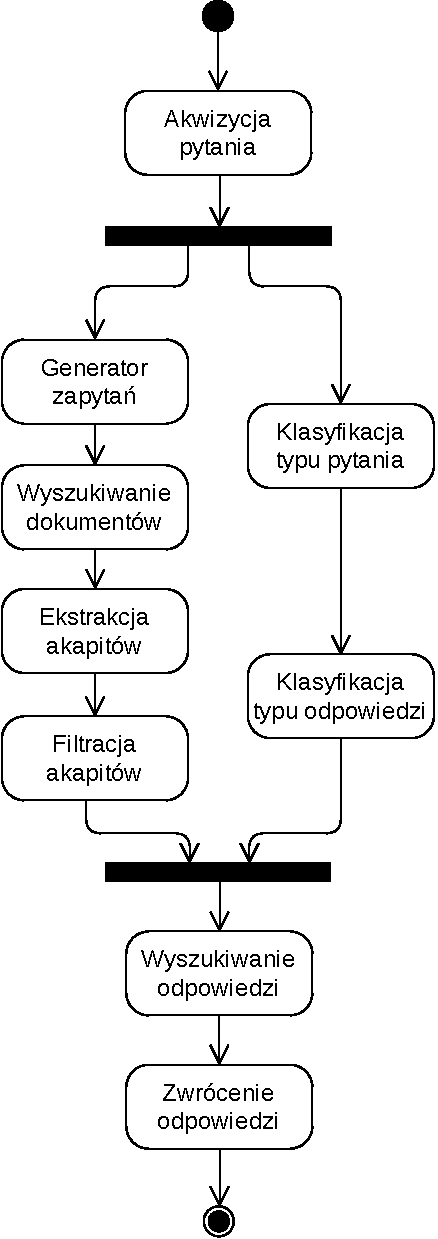
\includegraphics[width=0.7\columnwidth]{figures/WEDT-Algorytm.pdf}
    \caption{Ogólny schemat algorytmu odpowiadania na pytania}
    \label{fig:algorithm-overview}
\end{figure}

Pierwszym krokiem algorytmu jest akwizycja pytania od użytkownika systemu. Każde pytanie będzie analizowane w~sposób indywidualny, bez przechowywania wcześniejszych pytań i~utrzymywania kontekstu. Nie zakładamy również żadnego profilowania użytkowników, ponieważ typowo proste pytania o~fakty, są ze sobą słabo powiązane.

W~kolejnym kroku, strumień sterowania rozdwaja się i~jest przekazywany do dwóch modułów, które przetwarzają zapytanie równolegle. Moduł akwizycji wiedzy, na podstawie przekazanego pytania, stara się uzyskać jak największą ilość \emph{snippetów}, generując specjalistyczne zapytania do każdej z~czterech wyszukiwarek, tak jak to zostało przedstawione w~\cite{zheng2002answerbus}. Oprócz tego, aby wykorzystać redundantość sieci~WWW, do wyszukiwarek wysłane zostaną również okrojone zapytania, pozbawione części słów, tak aby zwiększyć zakres poszukiwań, podobnie jak w~\cite{brill2002analysis}. Aby zwiększyć rozmiar zbioru wyszukanych \emph{snippetów}, słowa kluczowe w~zapytaniu, będą wymieniane na ich synonimy~\cite{przybyla-2013-question}.

W~trakcie wyszukiwania \emph{snippetów}, w~drugiej gałęzi algorytmu, następuję klasyfikacja typu pytania i~oczekiwanej odpowiedzi. Klasy pytań są definiowane przez zaimki pytające. Wyróżniamy pytania typu: \emph{Kto?}, \emph{Jaki/Jaka/Jakie?}, \emph{Jak?}, \emph{Gdzie?}, \emph{Kiedy?}, \emph{Co?} oraz \emph{Który/Która/Które?}. Wykrywanie typu pytania odbywać się będzie w~prosty sposób, stosując reguły podstawieniowe oraz rozkład zdania. Określanie typu oczekiwanej odpowiedzi będzie wynikało głównie z~typu pytania, wspartej możliwością odpytania usługi \emph{plWordNet}~\cite{MazPiaRudSzpaKedz:16} oraz dodatkowym sprawdzeniem wyrażeń regularnych.

Każdy wyszukany \emph{snippet} zostanie poddany analizie morfologicznej, po której przyporządkowana zostanie mu odpowiednia ocena. W~każdym zdaniu, za pomocą taggera oraz \emph{plWordNetu} wyszukiwane będą \emph{Named-Entities}, które mogą stanowić potencjalną odpowiedź na pytanie. Ostatnim krokiem procesu będzie zwrócenie najlepszej odpowiedzi lub zbioru najlepszych odpowiedzi. Do odpowiedzi dołączony może zostać link ze źródłem, w~celu umożliwienia użytkownikowi systemu osobistej weryfikacji odpowiedzi.

\subsection{Dekompozycja systemu}
Zaprojektowany system składa się z~kilku funkcjonalnych komponentów, z~czego tylko część zostanie przez nas zrealizowana w~całości. Duży fragment systemu będzie wykorzystywał gotowe komponenty takie jak \emph{plWordNet} czy wyszukiwarki internetowe. Na rysunku \ref{fig:system-components} przedstawiony został podział na komponenty funkcjonalne, ze szczególnym wyróżnieniem relacji pomiędzy nimi.

\begin{figure}[h]
    \centering
    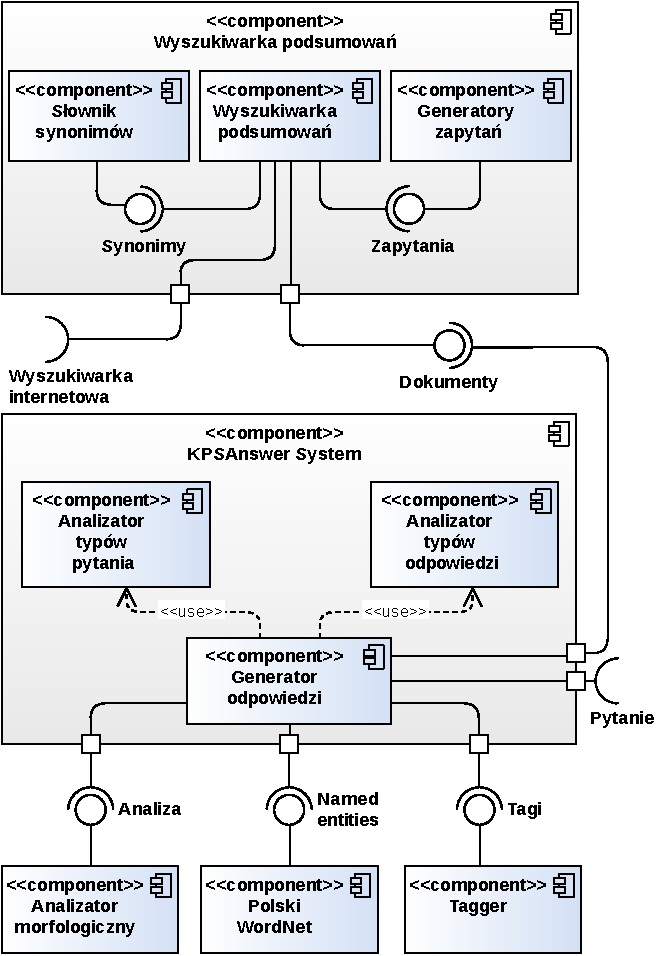
\includegraphics[width=\columnwidth]{figures/WEDT-Komponenty.pdf}
    \caption{Podział systemu KPSAnswer na funkcjonalne komponenty}
    \label{fig:system-components}
\end{figure}

Planowany podział zakłada istnienie dwóch, głównych komponentów:
\emph{KPSAnswer System\footnote{Nazwa KPS pochodzi od pierwszych liter nazwisk autorów}} oraz wyszukiwarki podsumowań, wspieranych kilkoma komponentami pobocznymi.
Komponent \emph{KPSAnswer System} zajmuje się generacją odpowiedzi na pytania przychodzące z~zewnątrz, korzystając z~interfejsu \texttt{Pytania}. W~celu wygenerowania odpowiedzi, komponent ten odpytuje \texttt{Wyszukiwarkę podsumowań} przy użyciu interfejsu \texttt{Dokumenty} o~zbiór podsumowań, mogących zawierać odpowiedź. \texttt{Wyszukiwarka podsumowań} zdobywa podsumowania odpytując strony implementujące interfejs \texttt{Wyszukiwarka internetowa}.

\subsection{Propozycja implementacji}
Wydzielenie dwóch głównych komponentów, komunikujących się z~komponentami pobocznymi za pomocą interfejsów komunikujących, pozwala na wydzielenie bytów, aplikacji w~systemie. Proponowany przez nas podział na aplikacje, przedstawiony został na rysunku~\ref{fig:system-deployment}.

\begin{figure}[h!]
    \centering
    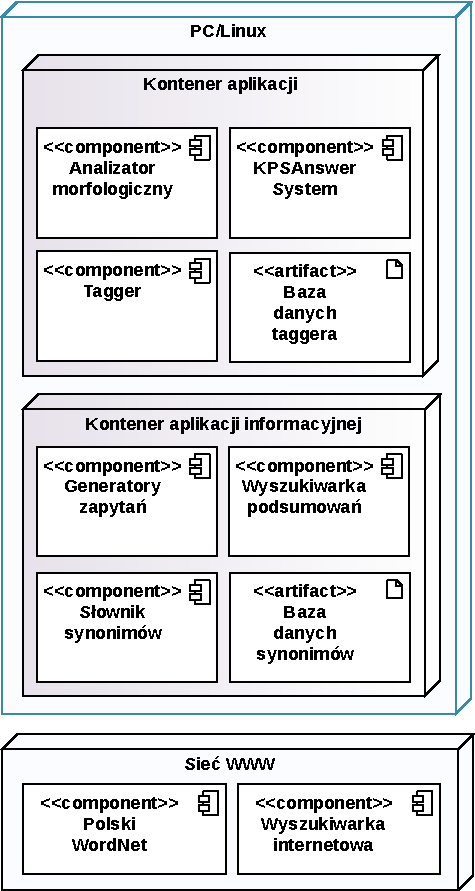
\includegraphics[width=0.8\columnwidth]{figures/WEDT-Deployment.pdf}
    \caption{Diagram rozmieszczenia systemu KPSAnswer}
    \label{fig:system-deployment}
\end{figure}

Na maszynie PC z~systemem operacyjnym Linux uruchomione zostaną dwa procesy. Pierwszy z~nich będzie przyjmował pytania za pomocą wystawionego interfejsu REST API. Dzięki temu, aplikacja będzie mogła być odpytywana za pomocą wiersza poleceń, programów typu Postman lub dedykowanego interfejsu graficznego. Drugi proces odpowiedzialny będzie za przeszukiwanie sieci WWW, generację odpowiednich zapytań oraz odpytywanie wyszukiwarek i~agregację podsumowań. Obie aplikacje będą komunikowały się z~aplikacjami w~sieci WWW, dlatego też maszyna będzie musiała być cały czas podłączona do internetu.  

\section{Dane testowe}
\label{sec:dane-testowe}
W~celu weryfikacji poprawności naszego rozwiązania, przygotowaliśmy zbiór danych testowych, składający się ponad 250 pytań o~ogólnej tematyce. Przygotowując pytania, staraliśmy się równomiernie podzielić zbiór pomiędzy pięć typów potencjalnej odpowiedzi. Pytania pochodziły głównie z~popularnych teleturniejów takich jak Milionerzy czy Jeden z~dziesięciu ale również z~innych popularnych quizów internetowych oraz konkursów wiedzy dla młodzieży.

\begin{figure}[h!]
    \begin{tikzpicture}
        \pie [rotate = 180]
        {20.3/OSOBA,
         19.9/MIEJSCE,
         19.6/DATA,
         20.3/WIELKOŚĆ,
         19.9/RZECZ}
    \end{tikzpicture}
    \label{fig:rozklad-typow-odpowiedzi}  
    \caption{Rozkład typów oczekiwanych odpowiedzi w~przygotowanej bazie pytań}
\end{figure}

Z~powodu charakteru pytań o~fakty, większość oczekiwanych odpowiedzi to rzeczowniki lub liczebniki. Oprócz tego, pojawią się również pytania o~cechy: przymiotniki i~przysłówki.

Duży zbiór danych pozwoli nam na przeprowadzenie badań nad poprawnością odpowiedzi systemu. Oprócz gotowego systemu, powstanie moduł badający procent poprawnych odpowiedzi w~sposób automatyczny. Aby tak badać poprawność, moduł ten musi mieć dostęp do poprawnych odpowiedzi. Co więcej, odpowiedź w~systemie powinna być przechowywana we wszystkich możliwych formach, ponieważ system może zwracać odpowiedź w~dowolnym przypadku, osobie czy liczbie. Problem ten został szerzej opisany w~artykule~\cite{brill2002analysis}.

Węzeł do automatycznego badania poprawności odpowiedzi pozwoli nam na przeprowadzenie dodatkowych badań nad zasadnością pewnych elementów w~systemie oraz wartości parametrów modułów. Modularność projektowanego systemu pozwoli nam na wyłączanie pewnych komponentów takich jak słownik synonimów, dzięki czemu będziemy mogli znaleźć optymalny kompromis pomiędzy dokładnością odpowiedzi a~czasem oczekiwania na odpowiedź.

\begin{figure}[h!]
    \begin{tikzpicture}
        \pie [rotate = 180]
        {62.5/Rzeczowniki,
         29.8/Liczebniki,
         7.7/Przymiotniki/przysłówki}
    \end{tikzpicture}
    \label{fig:rozklad-typow-odpowiedzi2}  
    \caption{Rozkład części mowy oczekiwanych odpowiedzi w~przygotowanej bazie pytań}
\end{figure}

\section{Podsumowanie}
\label{sec:podsumowanie}
W ramach etapu przeprowadzone zostały studia literaturowe na temat systemów odpowiadania na pytania. Na ich podstawie określono zakres projektu, tj. zaprojektowanie i implementacja własnego systemu odpowiadającego na pytania ogólne o określonych typach odpowiedzi (osoba, miejsce, data, cechy wielkościowe, przedmiot) zadane w języku polskim. W raporcie przedstawiono projekt rozwiązania oraz zarys algorytmu odpowiadania na pytania.  Na ich podstawie dokonana została dekompozycja tworzonego systemu. Wyszczególnione zostały komponenty do samodzielnej implementacji, a także wskazano, z jakich gotowych modułów będzie składał się system. Na bazie wydzielonych komponentów przedstawiona została propozycja podziału systemu na aplikację. Na koniec opisano przygotowane dane testowe, zawierające 250 pytań i odpowiedzi.


Stworzona koncepcja systemu umożliwia jego skalowalność w przyszłości. Po zakończeniu projektu można będzie go dalej rozwijać poprzez dodawanie kolejnych obsługiwanych typów odpowiedzi, a także ulepszać przez wykorzystywane nowych modułów zewnętrznych.  Decyzja o wyborze języka polskiego jako język zadawania pytań i udzielania odpowiedzi zwiększa, naszym zdaniem, atrakcyjność systemu, z uwagi na niewielką ilość dostępnych rozwiązań w tym języku. Dodatkowym walorem dla nas jest także sposobność przetestowania istniejących narzędzi dla języka polskiego.

\bibliographystyle{abbrv}
\bibliography{bibliography}

\end{document}